\chapter{Soporte software del robot}
\label{cap:capitulo6}

\begin{flushright}
\begin{minipage}[]{10cm}
\emph{El software es una gran combinación entre arte e ingeniería}\\
\end{minipage}\\

Bill Gates\\
\end{flushright}

\vspace{1cm}

Escribe aquí un párrafo explicando brevemente 

\section{}

Capítulo 6: incluir lo de openvision paper\\
capitulo 7: explicar experimentos impresora del instituto \\

\section{Snippets}

Puede resultar interesante, para clarificar la descripción, mostrar fragmentos de código (o \textit{snippets}) ilustrativos. En el Código \ref{cod:codejemplo} vemos un ejemplo escrito en \texttt{C++}.

\begin{code}[h]
	\begin{lstlisting}[language=C++]
		void Memory::hypothesizeParallelograms () {
			for(it1 = this->controller->segmentMemory.begin(); it1++) {
				squareFound = false; it2 = it1; it2++;
				while ((it2 != this->controller->segmentMemory.end()) && (!squareFound)) {
					if (geometry::haveACommonVertex((*it1),(*it2),&square)) {
						dist1 = geometry::distanceBetweenPoints3D ((*it1).start, (*it1).end);
						dist2 = geometry::distanceBetweenPoints3D ((*it2).start, (*it2).end);
					}
					// [...]
				\end{lstlisting}
				\caption[Función para buscar elementos 3D en la imagen]{Función para buscar elementos 3D en la imagen}
				\label{cod:codejemplo}
			\end{code}
			
			En el Código \ref{cod:codejemplo2} vemos un ejemplo escrito en \texttt{Python}.
			
			\begin{code}[h]
				\begin{lstlisting}[language=Python]
					def mostrarValores():
					print (w1.get(), w2.get())
					
					master = Tk()
					w1 = Scale(master, from_=0, to=42)
					w1.pack()
					w2 = Scale(master, from_=0, to=200, orient=HORIZONTAL)
					w2.pack()
					Button(master, text='Show', command=mostrarValores).pack()
					
					mainloop()
				\end{lstlisting}
				\caption[Cómo usar un Slider]{Cómo usar un Slider}
				\label{cod:codejemplo2}
			\end{code}
			
			\section{Verbatim}
			
			Para mencionar identificadores usados en el código ---como nombres de funciones o variables--- en el texto, usa el entorno literal o verbatim \verb|hypothesizeParallelograms()|. También se puede usar este entorno para varias líneas, como se ve a continuación:
			
			\begin{verbatim}
				void Memory::hypothesizeParallelograms () {
					// add your code here
				}
			\end{verbatim}
			
			\section{Ecuaciones}
			
			Si necesitas insertar alguna ecuación, puedes hacerlo. Al igual que las figuras, no te olvides de referenciarlas. A continuación se exponen algunas ecuaciones de ejemplo: Ecuación \ref{ec:ec1} y Ecuación \ref{ec:ec2}.
			
			\begin{myequation}[h]
				\begin{equation}
					H = 1 - \frac{\sum_{i=0}^{N}\frac{(\frac{d_{j_s} + d_{j_e}}{2})}{N}}{M}
					\nonumber
					\label{ec:ec1}
				\end{equation}
				\caption[Ejemplo de ecuación con fracciones]{Ejemplo de ecuación con fracciones}
			\end{myequation} 
			
			\begin{myequation}[h]
				\begin{equation}
					v(entrada)= \left\{
					\begin{array}{lcc}
						0 & \mbox{if} & \epsilon_t < 0.1\\
						K_p\cdot{(T_{t}-T)} & \mbox{if}& 0.1 \leq \epsilon_t < M_t\\
						K_p \cdot M_t & \mbox{if}& M_t < \epsilon_t
					\end{array}
					\right.
					\label{ec:ec2}
				\end{equation}
				\caption[Ejemplo de ecuación con array y letras y símbolos especiales]{Ejemplo de ecuación con array y letras y símbolos especiales}
			\end{myequation}
			
			\section{Tablas o cuadros}
			
			Si necesitas insertar una tabla, hazlo dígnamente usando las propias tablas de \LaTeX, no usando pantallazos e insertándolas como figuras... En el Cuadro \ref{cuadro:ejemplo} vemos un ejemplo.
			
			\begin{table}[H]
				\begin{center}
					\begin{tabular}{|c|c|}
						\hline
						\textbf{Parámetros} & \textbf{Valores} \\
						\hline
						Tipo de sensor & Sony IMX219PQ[7] CMOS 8-Mpx \\
						Tamaño del sensor & 3.674 x 2.760 mm (1/4" format) \\
						Número de pixels & 3280 x 2464 (active pixels) \\
						Tamaño de pixel & 1.12 x 1.12 um \\
						Lente & f=3.04 mm, f/2.0 \\
						Ángulo de visión & 62.2 x 48.8 degrees \\
						Lente SLR equivalente & 29 mm \\
						\hline
					\end{tabular}
					\caption{Parámetros intrínsecos de la cámara}
					\label{cuadro:ejemplo}
				\end{center}
			\end{table}
			
			En los textos puedes poner palabras en \textit{cursiva}, para aquellas expresiones en sentido \textit{figurado}, palabras como \textit{robota}, que está fuera del diccionario castellano, o bien para resaltar palabras de una colección: \textit{(a)} es la primera letra del abecedario, \textit{(b)} es la segunda, etc.\\
			
			Al poner las dos líneas del anterior párrafo, este aparecerá separado del anterior. Si no las pongo, los párrafos aparecerán pegados. Sigue el criterio que consideres más oportuno.
			
			\section{Segunda sección}
			\label{sec:segundaseccion}
			
			No olvides incluir imágenes y referenciarlas, como la Figura \ref{fig:roomba}.
			
			\begin{figure} [h!]
				\begin{center}
					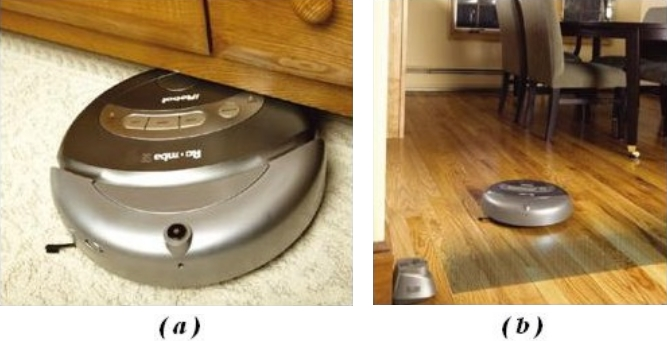
\includegraphics[width=8cm]{figs/roomba}
				\end{center}
				\caption{Robot aspirador Roomba de iRobot.}
				\label{fig:roomba}
			\end{figure}\
			
			Ni tampoco olvides de poner las URLs como notas al pie. Por ejemplo, si hablo de la Robocup\footnote{\url{http://www.robocup.org}}.
			
			\subsection{Números}
			\label{sec:subseccion}
			
			En lugar de tener secciones interminables, como la Sección \ref{sec:robotica}, divídelas en subsecciones.
			
			Para hablar de números, mételos en el entorno \textit{math} de \LaTeX, por ejemplo, $1.5Kg$. También puedes usar el símbolo del Euro como aquí: 1.500\euro.
			
			\subsection{Listas}
			
			Cuando describas una colección, usa \texttt{itemize} para ítems o \texttt{enumerate} para enumerados. Por ejemplo:
			
			\begin{itemize}
				\item \textit{Entorno de simulación.} Hemos usado dos entornos de simulación: uno en 3D y otro en 2D.
				\item \textit{Entornos reales.} Dentro del campus, hemos realizado experimentos en Biblioteca y en el edificio de Gestión.
			\end{itemize}\
			
			\begin{enumerate}
				\item Primer elemento de la colección.
				\item Segundo elemento de la colección.
			\end{enumerate}\
			
			\paragraph{Referencias bibliográficas}
			\label{sec:referencias}
			
			Cita, sobre todo en este capítulo, referencias bibliográficas que respalden tu argumento. Para citarlas basta con poner la instrucción \verb|\cite| con el identificador de la cita. Por ejemplo: libros como \cite{vega12e}, artículos como \cite{vega19b}, URLs como \cite{vega19a}, tesis como \cite{vega18b}, congresos como \cite{vega18a}, u otros trabajos fin de grado como \cite{vega08b}.
			
			Las referencias, con todo su contenido, están recogidas en el fichero \texttt{bibliografia.bib}. El contenido de estas referencias está en formato \texttt{BibTex}. Este formato se puede obtener en muchas ocasiones directamente, desde plataformas como \texttt{Google Scholar} u otros repositorios de recursos científicos.
			
			Existen numerosos estilos para reflejar una referencia bibliográfica. El estilo establecido por defecto en este documento es APA, que es uno de los estilos más comunes, pero lo puedes modificar en el archivo \texttt{memoria.tex}; concretamente, cambiando el campo \verb|apalike| a otro en la instrucción \verb|\bibliographystyle{apalike}|. 
			
			\
			
			\
			
			\
			
			Y, para terminar este capítulo, resume brevemente qué vas a contar en los siguientes.


\section{Corrector ortográfico}

Una vez tengas todo, no olvides pasar el corrector ortográfico de \LaTeX a todos tus ficheros \textit{.tex}. En \texttt{Windows}, el propio editor \texttt{TeXworks} incluye el corrector. En \texttt{Linux}, usa \texttt{aspell} ejecutando el siguiente comando en tu terminal:

\begin{verbatim}
aspell --lang=es --mode=tex check capitulo1.tex
\end{verbatim}
